\section{Dokumentation und Metadaten}

Die Datendokumentation und die Erstellung von Metadaten sind unerlässlich, um
Ihre Daten im Detail zu verstehen und auch anderen Forschenden zu helfen, Ihre
Daten zu finden, verstehen und weiter zu nutzen bzw. richtig zu zitieren. Jede
Disziplin hat eigene, spezifische Metadatenstandards, die Sie selber
nachschlagen müssen. Weitere allgemeine Leitlinien finden sie im folgenden Text.

\subsection{Wichtige Information beim Sammeln oder Erstellen von Daten}

\begin{itemize}
  \item Notieren Sie alle Dateinamen und -formate, die mit dem Projekt in
        Verbindung stehen, wie die Daten organisiert sind, wie die Daten
        erzeugt wurden (einschließlich aller verwendeten Geräte samt Software),
        und Informationen darüber, wie die Daten verändert oder verarbeitet
        wurden.
  \item Erläuterung von Computerprogrammen, Abkürzungen oder Variablen, die in
        den Daten oder in der Dateibenennungsstruktur verwendet werden.
  \item Notieren Sie, woher Sie die Daten haben, damit Sie und andere sie
        wiederfinden können.
\end{itemize}

\subsection{Dokumentation von Daten: Metadaten}\label{sc:data-documentation}

Das verwendete Metadatenschema folgt der Empfehlung des weltweiten DataCite-Konsortiums (TIB Hannover, Britische Bibliothek, Denmark Technical Information Center, ETH Zürich, CalTech, Australian National Data Service, ...).
Diese Daten sind in einer "readme.json" Datei in \textbf{JEDEM VERZEICHNIS} Ihrer Daten gespeichert! Sie können unseren 'Readme File Creator' (siehe \ref{fig:readme-creator}) nutzen, um diese Datei zu erzeugen. \\
\begin{wrapfigure}{r}{0.5\linewidth}
  \vspace{-1em}
  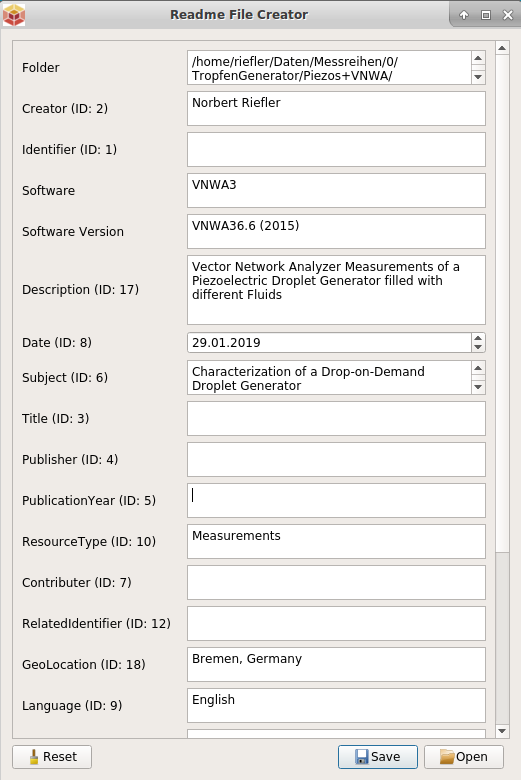
\includegraphics[width=\linewidth]{Figure02_ReadmeFileCreator.png}
  \caption{Data Input Tool: Readme-File-Creator}
  \label{fig:readme-creator}
\end{wrapfigure}
Im Folgenden werden einige der extrahierten Eigenschaften erläutert; weitere
Informationen finden Sie in Tabelle 3 in \cite{datacite2019}: \\[6pt]
%
\textbf{ID 1: Kennung} \\
Nummer, die zur Identifizierung der Daten verwendet wird. Dies kann ein DOI
(Digital Object Identifier) im Falle einer Veröffentlichung oder eine PID
(Persistent Identifier) aus dem ELN sein (eLabFTW  generiert eine lange Nummer
für jedes Experiment, siehe \ref{ssc:ELN} \nameref{ssc:ELN}). \\[6pt]
%
\textbf{ID 2: Erstellerin oder Ersteller} \\
Name der Person, die für die beschriebenen Daten verantwortlich ist (ORCID, Open Researcher Contributor Identification). \\[6pt]
%
\textbf{ID 3: Titel} \\
Kann der Titel eines Datensatzes, der Name einer Software oder der Titel eines
Artikels sein. \\[6pt]
%
\textbf{ID 4: Herausgeber} \\
Der Name der Einrichtung, die die Daten produziert, aufbewahrt, archiviert,
veröffentlicht, druckt, vertreibt, freigibt oder herausgibt (z.B.
"Leibniz-Institut für Werkstofforientierte Technologien - IWT"). \\[6pt]
%
\textbf{ID 5: Jahr der Veröffentlichung} \\
Das Jahr, in dem die Daten öffentlich zugänglich gemacht wurden oder werden. \\[6pt]
%
\textbf{ID 8: Datum} \\
Entstehungsdatum der Daten, einschließlich des Start- und Enddatums des
Projekts, des Datums der Datenänderung und des von den Daten abgedeckten. \\[6pt]
%
\textbf{ID 9: Sprache} \\
Sprache(n) des Inhalts der Quelle. \\[6pt]
%
\textbf{ID 10: Ressourcentyp} \\
Eine Beschreibung der Ressource; meist "DataSet", kann aber auch "\verb+Audiovisuell+",
"High-Speed Images", "DataPaper", etc. sein.\\[6pt]
%
\textbf{ID 19: Förderkennzeichen} \\
Organisationen oder Behörden, die die Forschung finanziert haben. \\[6pt]
%
\textbf{ID 16: Rechte} \\
Alle bekannten Rechte am geistigen Eigentum an den Daten. Die beste Wahl ist
normalerweise die Creative Commons Lizenz 'CC-BY' (BY attribution) oder 'CC-0'
für Daten sowie die 'CC Version 4.0' für schriftliche Dokumente. \\[6pt]
%
\textbf{ID 17: Beschreibung} \\
Wie die Daten erzeugt wurden, einschließlich der verwendeten Geräte oder
Software, des Versuchs\-protokolls und anderer Dinge, die Sie in ein Laborjournal
aufnehmen könnten. \\[6pt]
%
\textbf{ID 18: Geolokalisierung} \\
Wenn sich die Daten auf einen physischen Ort beziehen, halten Sie Informationen
über die geografische Abdeckung fest. \\[6pt]
%
Das oben in \autoref{fig:readme-creator} abgebildete Tool kann vom VT-Server (/VT-Allgemein/Software/ReadmeFile- Creator) für jedes Betriebssystem  heruntergeladen werden, um die Eingabe von Metadaten zu vereinfachen. Sie  können automatisch eine Datei namens 'readme.json' mit Ihren Metadaten, eingebettet in ein JSON (Java Scipt Object Notation)-Format, erstellen, die sowohl als Dokumentation als auch als Metadaten für Data Science Methods verwendet wird. Diese Datei wird in jedem Verzeichnis gespeichert, das Daten oder Programmcode enthält.\\
%
Dieselbe DataCite-Metadaten-Struktur kann auch im JSON-Editor des ELNs (siehe \ref{ssc:ELN}) abgebildet bzw. eingegeben werden.
